\documentclass{article}
\usepackage[utf8]{inputenc}
\usepackage[english, ukrainian]{babel}
\usepackage{fontsize}
\usepackage{geometry}
\usepackage{amsthm}
\usepackage{amsfonts}
\usepackage{graphicx}
\usepackage[ruled]{algorithm2e}
\usepackage{hyperref}
\usepackage{biblatex}
\usepackage{csquotes}
\usepackage{mathtools}
\usepackage{amsmath}
\usepackage{amssymb}
\usepackage{bbm}
\usepackage{tabularx}
\usepackage{xcolor}

\usepackage{tikz}
\usetikzlibrary{decorations.pathmorphing}

\usepackage{enumitem}
\usepackage{nicefrac}

\usepackage{listings}
\definecolor{codegreen}{rgb}{0,0.6,0}
\definecolor{codegray}{rgb}{0.5,0.5,0.5}
\definecolor{codepurple}{rgb}{0.58,0,0.82}
\definecolor{backcolour}{rgb}{0.95,0.95,0.92}

\lstdefinestyle{mystyle}{
    backgroundcolor=\color{backcolour},   
    commentstyle=\color{codegreen},
    keywordstyle=\color{magenta},
    numberstyle=\tiny\color{codegray},
    stringstyle=\color{codepurple},
    basicstyle=\ttfamily\footnotesize,
    breakatwhitespace=false,         
    breaklines=true,                 
    captionpos=b,                    
    keepspaces=true,                 
    numbers=left,                    
    numbersep=5pt,                  
    showspaces=false,                
    showstringspaces=false,
    showtabs=false,                  
    tabsize=2
}

\lstset{style=mystyle}
\hypersetup{colorlinks=true, linkcolor=[RGB]{255, 3, 209}, citecolor={black}}

\graphicspath{ {../Images/} }

\begin{document}
    \begin{titlepage}
        \begin{center}
            \begin{center}
                НАЦІОНАЛЬНИЙ ТЕХНІЧНИЙ УНІВЕРСИТЕТ УКРАЇНИ
                «КИЇВСЬКИЙ ПОЛІТЕХНІЧНИЙ ІНСТИТУТ імені Ігоря СІКОРСЬКОГО»

                Фізико-технічний інститут
            \end{center}
        $\newline$
        \vspace{3.3cm}
        
        {
        РОЗРАХУНКОВО-ГРАФІЧНА РОБОТА
        
        з кредитного модуля «Методи обчислень»
        
        на тему:
        
        «ОБЧИСЛЮВАЛЬНЕ РОЗВ’ЯЗАННЯ ДИФЕРЕНЦІАЛЬНИХ
        
        РІВНЯНЬ У ЧАСТИННИХ ПОХІДНИХ»
        
        Варіант №10
        }
        \vspace{3cm}
        \begin{flushright}
            Виконав\\студент 3 курсу ФТІ\\групи ФІ-21\\Климентьєв Максим Андрійович
            
            \vspace{1cm}

            Перевірив:\\\underline{\hspace{5cm}}\\Оцінка:\\\underline{\hspace{5cm}}
        \end{flushright}
        \vspace{3.5cm}
        Київ --- 2025
        \end{center}
    \end{titlepage}
    \newpage

    \pagenumbering{gobble}
    \tableofcontents
    \cleardoublepage
    \pagenumbering{arabic}
    \setcounter{page}{3}

    \newpage
    \section{ПОСТАНОВКА ЗАДАЧІ}
    \textbf{Варіант 10}

    Знайти чисельний розв’язок рівняння коливань струни:

    $$ \frac{\partial^2{u}}{\partial{t^2}} = \frac{\partial^2{u}}{\partial{x^2}} + F(t, x) $$
    % $$ u_{tt} = u_{xx} + F(t, x) $$
    $$ 0 < x < L = 1 $$
    % $$ u \vert_{(t = 0)} = u_0 = x \cdot (x+1) $$
    $$ u(t = 0) = u_0 = x \cdot (x+1) $$
    % $$ \frac{\partial{u}}{\partial{t}} \vert_{(t = 0)} = 0 $$
    $$ \frac{\partial{u}}{\partial{t}}(t = 0) = 0 $$
    % $$ u\vert_{t = 0} = u_1(t) $$
    $$ u(t, 0) = u_1(t) $$
    % $$ u\vert_{t = L} = u_2(t) $$
    $$ u(t, L) = u_2(t) $$

    \hrule

    $$ u(t,x) = u_0(x) \cdot \cos(\pi \cdot t) $$
    $$ u_0(x) = u_0 = x \cdot (x+1) $$
    $$ u(t,x) = x \cdot (x+1) \cdot \cos(\pi \cdot t) $$

    \hrule

    $$ u(t,0) = 0 \cdot 1 \cdot \cos(\pi \cdot t) = 0 $$
    $$ u(t, L) = L \cdot (L+1) \cdot \cos(\pi \cdot t) = 1 \cdot 2 \cdot \cos(\pi \cdot t) = 2 \cdot \cos(\pi \cdot t) $$

    \hrule

    $$ \frac{\partial{u}}{\partial{x}} = 2 \cdot x \cdot \cos(\pi \cdot t) + \cos(\pi \cdot t) $$
    $$ \frac{\partial^2{u}}{\partial{x^2}} = 2 \cdot \cos(\pi \cdot t) $$

    $$ \frac{\partial{u}}{\partial{t}} = -\pi \cdot x \cdot (x+1) \cdot \sin(\pi \cdot t) $$
    $$ \frac{\partial^2{u}}{\partial{t^2}} = -\pi^2 \cdot x \cdot (x+1) \cdot \cos(\pi \cdot t) $$

    \hrule

    $$ \frac{\partial^2{u}}{\partial{t^2}} = \frac{\partial^2{u}}{\partial{x^2}} + F(t, x) $$
    $$ \frac{\partial^2{u}}{\partial{t^2}} - \frac{\partial^2{u}}{\partial{x^2}} = F(t, x) $$
    $$ F(t, x) = -\pi^2 \cdot x \cdot (x+1) \cdot \cos(\pi \cdot t) - 2 \cdot \cos(\pi \cdot t) $$
    $$ F(t, x) = -\cos(\pi \cdot t) \cdot \left(\pi^2 \cdot x \cdot (x+1) + 2\right) $$

    \hrule

    Навести приклади процесів, які моделюються за допомогою диференціальних рівнянь у частинних похідних гіперболічного типу
    
    \newpage
    \section{ОГЛЯД ТА АНАЛІЗ ІСНУЮЧИХ МЕТОДІВ ЧИСЕЛЬНОГО РОЗВ’ЯЗАННЯ ДРЧП}
    \newpage
    \section{ДОСЛІДЖЕННЯ УМОВ ЗАСТОСУВАННЯ ОБРАНОГО МЕТОДУ}

        Явна схема

        $$ \frac{u_i^{k+1} - 2 \cdot u_i^{k} + u_i^{k-1}}{\Delta{t}^2} = \frac{u_{i+1}^{k} - 2 \cdot u_i^{k} + u_{i-1}^{k}}{\Delta{x}^2} + F_i^{k} $$
        $$ u_i^{k+1} - 2 \cdot u_i^{k} + u_i^{k-1} = \Delta{t}^2 \cdot \left( \frac{u_{i+1}^{k} - 2 \cdot u_i^{k} + u_{i-1}^{k}}{\Delta{x}^2} + F_i^{k} \right) $$
        $$ u_i^{k+1} = 2 \cdot u_i^{k} - u_i^{k-1} + \Delta{t}^2 \cdot \left( \frac{u_{i+1}^{k} - 2 \cdot u_i^{k} + u_{i-1}^{k}}{\Delta{x}^2} + F_i^{k} \right) $$
        $$ u(i, k+1) = 2 \cdot u(i, k) - u(i, k-1) + \Delta{t}^2 \cdot \left( \frac{u(i+1, k) - 2 \cdot u(i, k) + u(i-1, k)}{\Delta{x}^2} + F(i, k) \right) $$

        Явно-неявна схема (тришарова схема з вагами)

        \begin{equation*}
            \begin{split}
                \frac{u_i^{k+1} - 2 \cdot u_i^{k} + u_i^{k-1}}{\Delta{t}^2} & = \sigma_1 \left( \frac{u_{i+1}^{k+1} - 2 \cdot u_i^{k+1} + u_{i-1}^{k+1}}{\Delta{x}^2} + F_i^{k+1} \right) +\\
                & + (1 - \sigma_1 - \sigma_2) \left( \frac{u_{i+1}^{k} - 2 \cdot u_i^{k} + u_{i-1}^{k}}{\Delta{x}^2} + F_i^{k} \right) +\\
                & + \sigma_2 \left( \frac{u_{i+1}^{k-1} - 2 \cdot u_i^{k-1} + u_{i-1}^{k-1}}{\Delta{x}^2} + F_i^{k-1} \right)\\
            \end{split}
        \end{equation*}

        $$ u \vert_{(t = 0)} = u_0 = x \cdot (x+1) $$
        $$ \frac{\partial{u}}{\partial{t}} \vert_{(t = 0)} = 0 $$
        % $$ \frac{u^1 - u^0}{\Delta{t}} = u_{10} \rightarrow u^1 $$
        $$ A\left(u^{k+1}\right) = B\left(u^k, u^{k-1}\right) \rightarrow \text{СЛАР або СНАР} $$

    \newpage
    \section{ОПИС ПРОГРАМНОЇ РЕАЛИЗАЦІЇ}
        Параметри:

        Кількість вузлів $ x = 100 $
        
        Кількість індексів дискретного часу $ t = 100 000 $
        
        Відстань між сусідніми просторовими вузлами $ \Delta{x} = 0.01 $
        
        Відстань між сусідніми моментами часу $ \Delta{t} = 0.00005 $

        $ L = 1 $

%         \begin{lstlisting}[language=Python, caption=u0]
% def u0(x):
%     return x * (x + 1)
%         \end{lstlisting}

%         \begin{lstlisting}[language=Python, caption=u2]
% def u2(t):
%     return u0(L) * np.cos(np.pi * t)
%         \end{lstlisting}

%         \begin{lstlisting}[language=Python, caption=u]
% def u(t, x):
%     return u0(x) * np.cos(np.pi * t)
%         \end{lstlisting}

%         \begin{lstlisting}[language=Python, caption=F]
% def F(t, x):
%     return -np.cos(np.pi * t) * (np.pi**2 * x * (x + 1) + 2)
%         \end{lstlisting}

        Масиви, початковий та кінцевий \eqref{mat:xs}

        \begin{figure}[h!]
            % \centering
            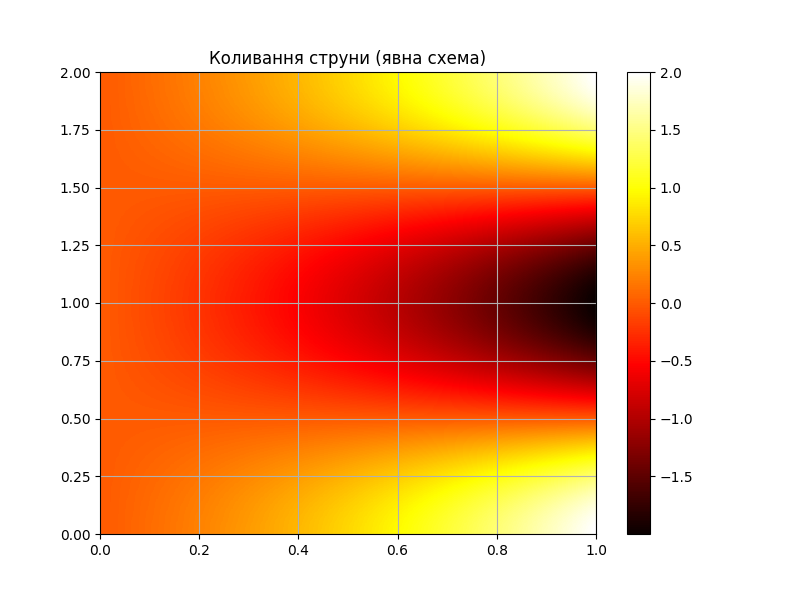
\includegraphics[width=0.5\linewidth]{straight_2d.png}
            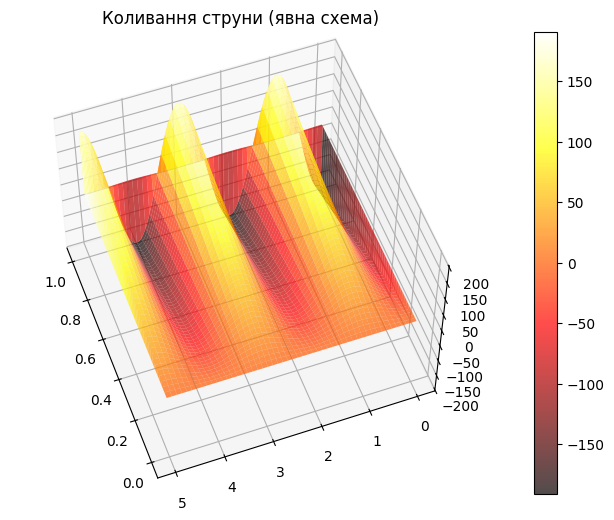
\includegraphics[width=0.5\linewidth]{straight_3d.png}
            \label{fig:2d_3d}
            \caption{2D and 3D}
        \end{figure}

    \newpage
    \section{ОГЛЯД МЕТОДІВ ПІДВИЩЕННЯ ТОЧНОСТІ}

        Тут здійснюється опис реалізації
        контрольного прикладу із зазначенням величин усіх параметрів, для яких
        проводились розрахунки (крок, початкові, кінцеві значення, критерії
        остановки ітераційних процедур (якщо такі є), значення коефіцієнтів
        рівняння, якщо такі конкретно не вказані в постановці задачі і т.п.). Також
        наводять опис результатів роботи програми (вивід масівів для різних кроків
        за часом для еволюційних задач, вивід масиву розв’язку для еліптичних
        задач). Основну масу числових результатів можна винести у додатки, аби не
        переобтяжувати текст розділу. Візуалізація результатів (побудова графіків та
        тривимірних поверхонь, що ілюструють поведінку процесу, що
        розглядається). Побудову графиків можна здійснювати як із використанням
        власної програми, так і застосовувати існуючі програмні продукти (Мathcad,
        Matlab та ін.) (рис.4.1).

    \newpage
    \section{ЗАСТОСУВАННЯ МЕТОДУ ПІДВИЩЕННЯ ТОЧНОСТІ ТА ЕФЕКТИВНОСТІ РОЗВ’ЯЗКУ ДО ПРИКЛАДУ РОБОТИ}
    \newpage
    \section{ВИСНОВКИ}
    \newpage
    \section{СПИСОК ВИКОРИСТАНИХ ДЖЕРЕЛ}
    \begin{enumerate}
        \item 
    \end{enumerate}
    \newpage
    \section{ДОДАТКИ}
        Різне

        Start Matrix (100000x100): 
        $$
        \left(\begin{matrix}
            0.0 & 0.01020304050607081 & 0.020610141822263034 & $\dots$ & 1.9697990001020307 & 2.0 \\
            0.0 & 0.0 & 0.0 & $\dots$ & 0.0 & 1.9999999753254956 \\
            0.0 & 0.0 & 0.0 & $\dots$ & 0.0 & 1.999999901301983 \\
            0.0 & 0.0 & 0.0 & $\dots$ & 0.0 & 1.9999997779294636 \\
            0.0 & 0.0 & 0.0 & $\dots$ & 0.0 & 1.9999996052079412 \\
            0.0 & 0.0 & 0.0 & $\dots$ & 0.0 & 1.9999993831374194 \\
            0.0 & 0.0 & 0.0 & $\dots$ & 0.0 & 1.9999991117179041 \\
            0.0 & 0.0 & 0.0 & $\dots$ & 0.0 & 1.9999987909494017 \\
            0.0 & 0.0 & 0.0 & $\dots$ & 0.0 & 1.9999984208319204 \\
            0.0 & 0.0 & 0.0 & $\dots$ & 0.0 & 1.9999980013654692 \\

            \dots & \dots & \dots & \dots & \dots & \dots \\

            0.0 & 0.0 & 0.0 & $\dots$ & 0.0 & -1.999999901301983 \\
            0.0 & 0.0 & 0.0 & $\dots$ & 0.0 & -1.9999999753254956 \\
            0.0 & 0.0 & 0.0 & $\dots$ & 0.0 & -2.0 \\
            \label{mat:xs}
        \end{matrix}\right)
        $$
    
        Received Matrix (100000x100): 
        $$
        \left(\begin{matrix}
            0.0 & 0.01020304050607081 & 0.020610141822263034 & $\dots$ & 1.9697990001020307 & 2.0 \\
            0.0 & -1.9999999805773505 & -3.9999507106768935 & $\dots$ & -188.43500752856792 & 1.9999999753254956 \\
            0.0 & -1.9999999065538376 & -3.9999998186151107 & $\dots$ & -195.91107678311408 & 1.999999901301983 \\
            0.0 & -1.9999997831813179 & -3.999999571870071 & $\dots$ & -195.99956337495996 & 1.9999997779294636 \\
            0.0 & -1.999999610459795 & -3.999999226427025 & $\dots$ & -196.0000441955736 & 1.9999996052079412 \\
            0.0 & -1.9999993883892728 & -3.9999987822859797 & $\dots$ & -196.00002406230797 & 1.9999993831374194 \\
            0.0 & -1.9999991169697569 & -3.999998239446947 & $\dots$ & -195.9999974666734 & 1.9999991117179041 \\
            0.0 & -1.9999987962012535 & -3.99999759790994 & $\dots$ & -195.99996603135077 & 1.9999987909494017 \\
            0.0 & -1.999998426083771 & -3.9999968576749736 & $\dots$ & -195.9999297598208 & 1.9999984208319204 \\
            0.0 & -1.9999980066173189 & -3.9999960187420682 & $\dots$ & -195.99988865209056 & 1.9999980013654692 \\

            \dots & \dots & \dots & \dots & \dots & \dots \\

            0.0 & 1.9999999065538376 & 3.9999998186151107 & $\dots$ & 195.9116714171308 & -1.999999901301983 \\
            0.0 & 1.9999999805773505 & 3.9999509606818933 & $\dots$ & 188.4918441248053 & -1.9999999753254956 \\
            0.0 & 0.0 & 0.0 & $\dots$ & 0.0 & -2.0 \\
            \label{mat:xr}
        \end{matrix}\right)
        $$

        % \includegraphics{}
        % \includegraphics{}
        % \includegraphics{}
        % \includegraphics{}

\end{document}